\documentclass[twocolumn]{article}
\usepackage[top=1.1in, left=0.85in, right=0.85in]{geometry}

% \usepackage{eclbkbox}
\usepackage{amsmath}
\usepackage{amssymb}
% \usepackage{code}
% \usepackage{amscd}
% \usepackage{xy}
\usepackage{graphicx}
% \usepackage{fancyhdr}
% \usepackage{color}
% \usepackage[dark,all,bottom,landscape,timestamp]{draftcopy}
% \usepackage{everypage}

% \pagestyle{empty}

% \usepackage{ulem}
% go back to italics for emphasis, though
% \normalem

\newcommand\sfrac[2]{{}\,^{#1}\!/{}\!_{#2}}

\begin{document} 

\title{New results in $\sfrac{k}{n}$ Power-Hours}
\author{Dr.~Tom~Murphy~VII~Ph.D.\thanks{
Copyright \copyright\ 2012 the Regents of the Wikiplia
Foundation. Appears in SIGBOVIK 2013 with the chagrin of the
Association for Computational Heresy; {\em IEEEEEE!} press,
Verlag-Verlag volume no.~0x40-2A.
\yen 0.00}
}

\renewcommand\>{$>$}
\newcommand\<{$<$}

\date{1 April 2011}

\maketitle

\begin{abstract}
Something about the k-n hours

\end{abstract}

\vspace{1em}
{\noindent \small {\bf Keywords}:
  generalized binge drinking, maths,
  finite-state automata,
  abstract interpretation
}

\section*{Introduction}
Here's where I tell you about doo-dah and so-so.


\begin{figure}
\begin{center}
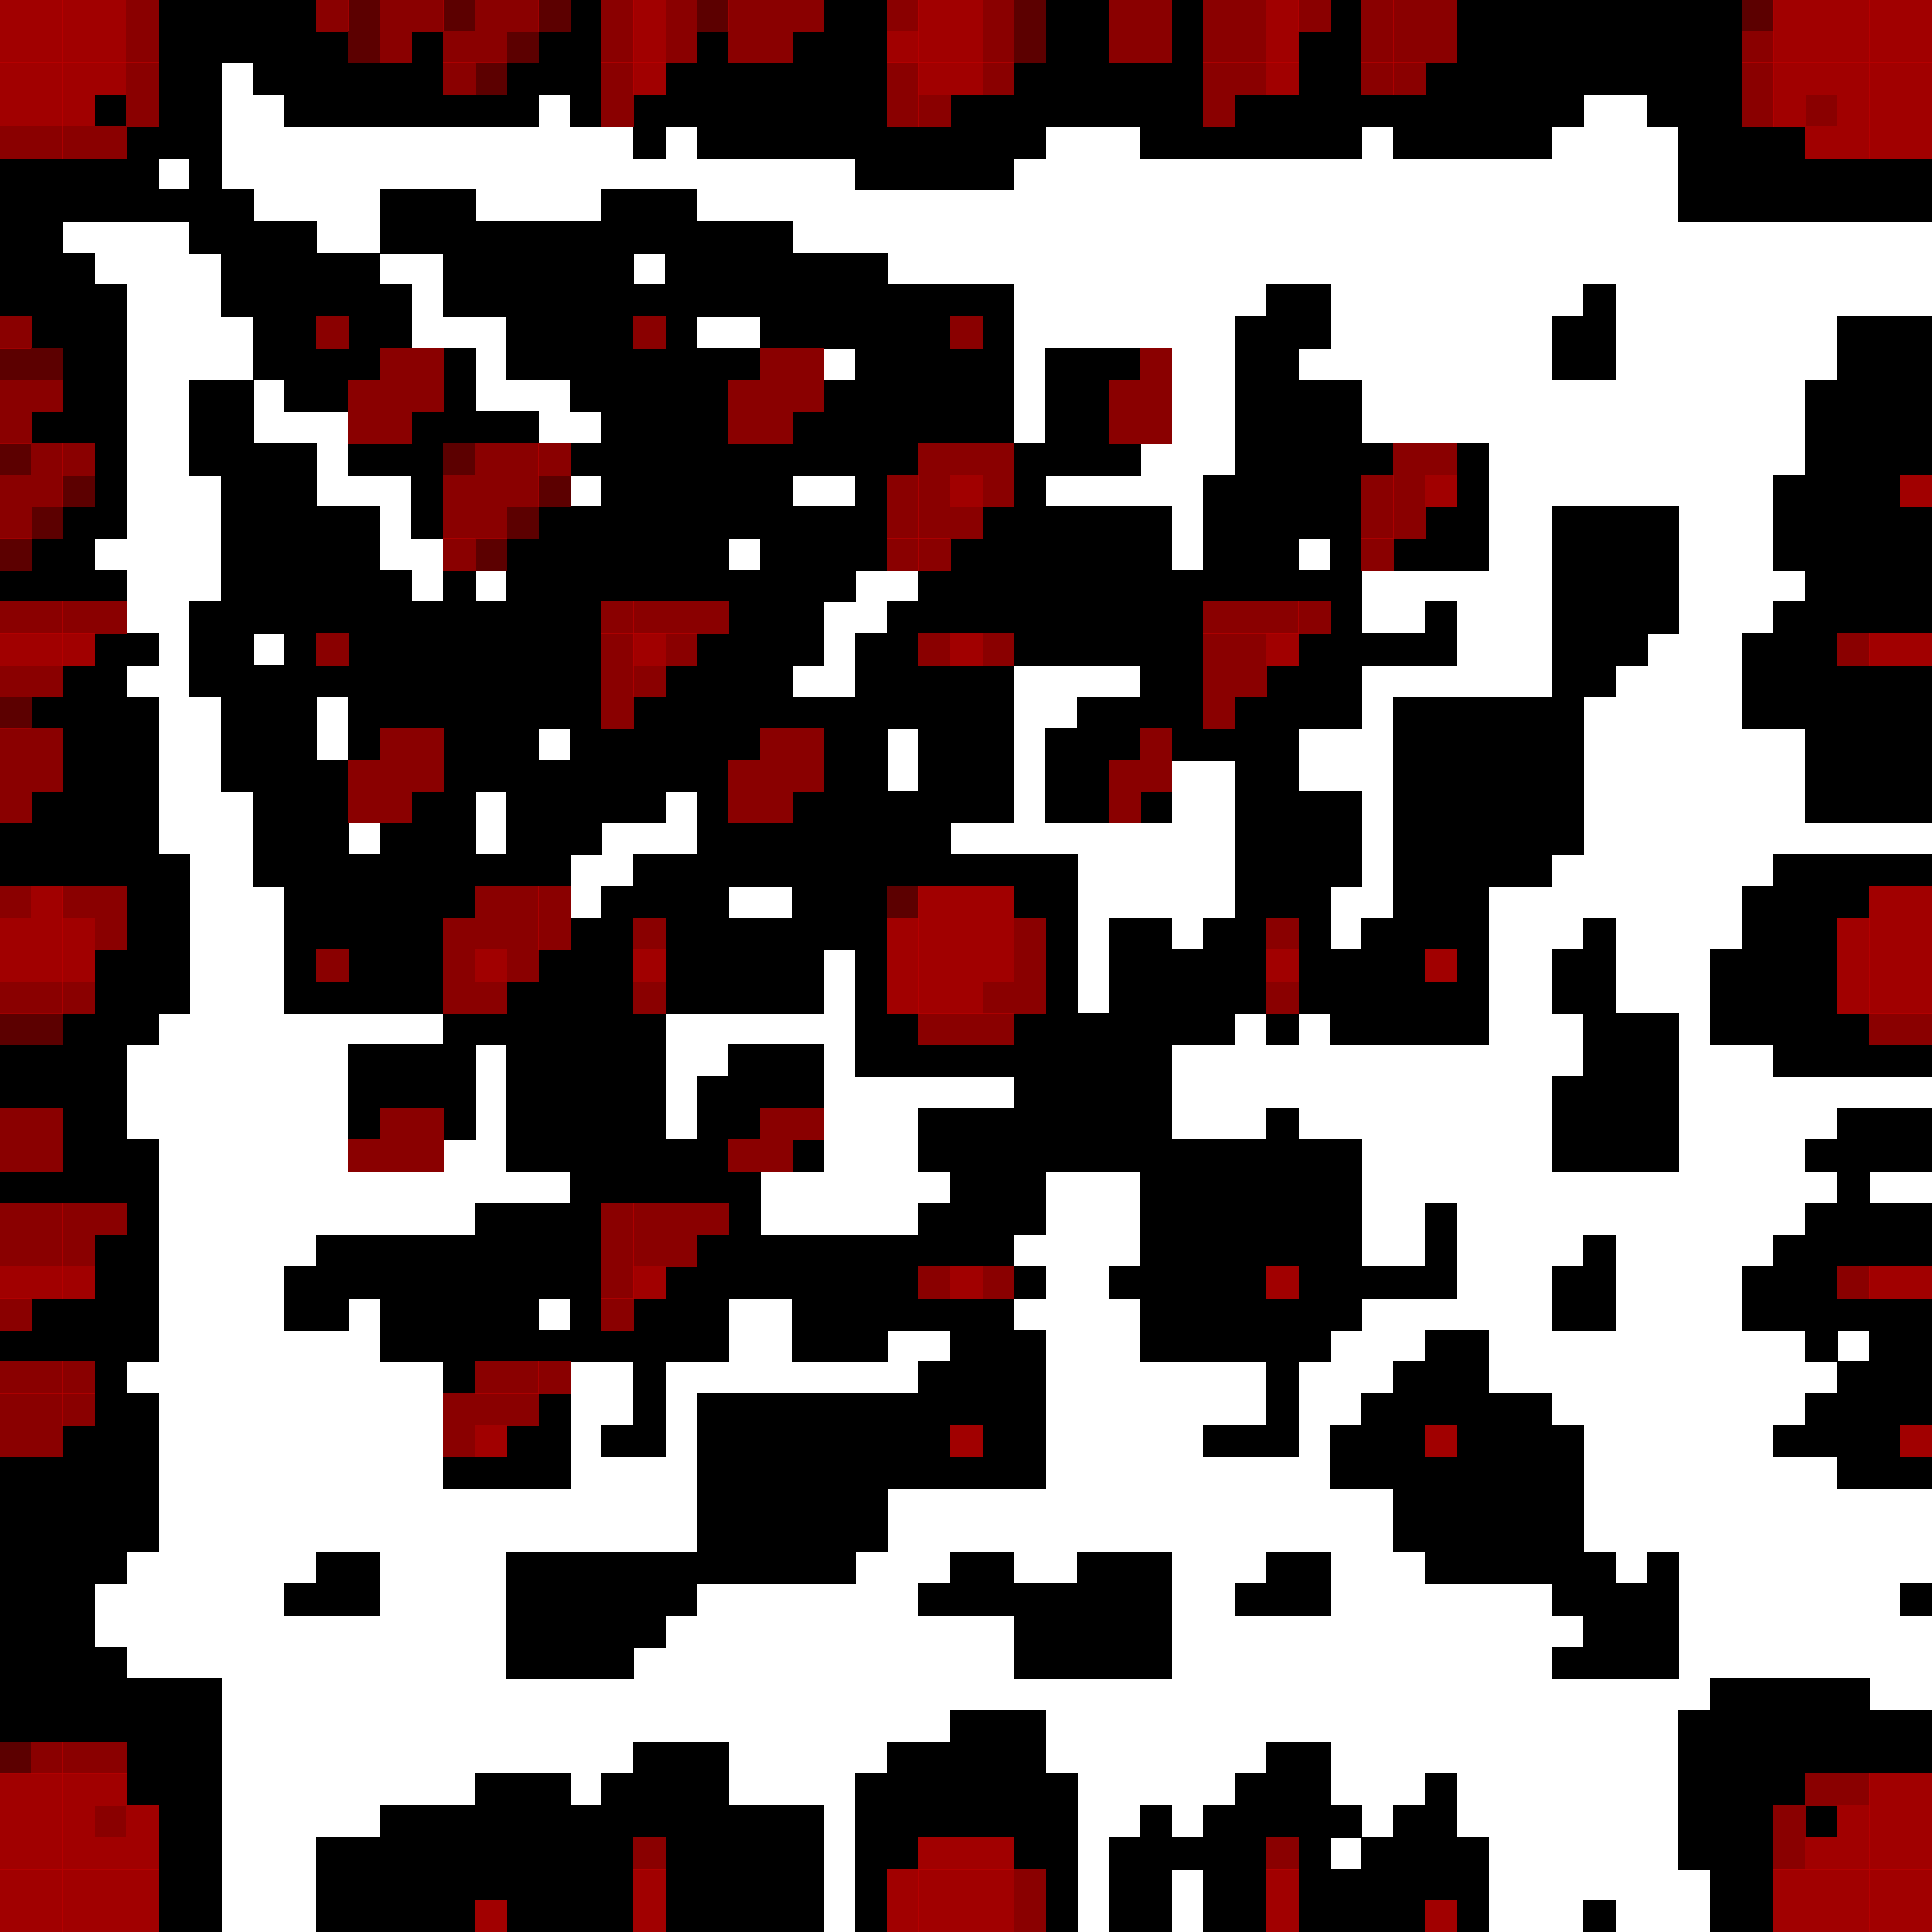
\includegraphics[width=0.90 \linewidth]{3and2.pdf}
\end{center}\vspace{-0.1in}
\caption{Outcomes possible for the first two players in all different
  3-player power hours (black), overlayed by all possible outcomes
  outcomes for 2-player power hours (red). Mainly included because
  it looks pretty sweet.
}
\label{fig:3and2}
\end{figure}

\begin{figure}
\begin{center}
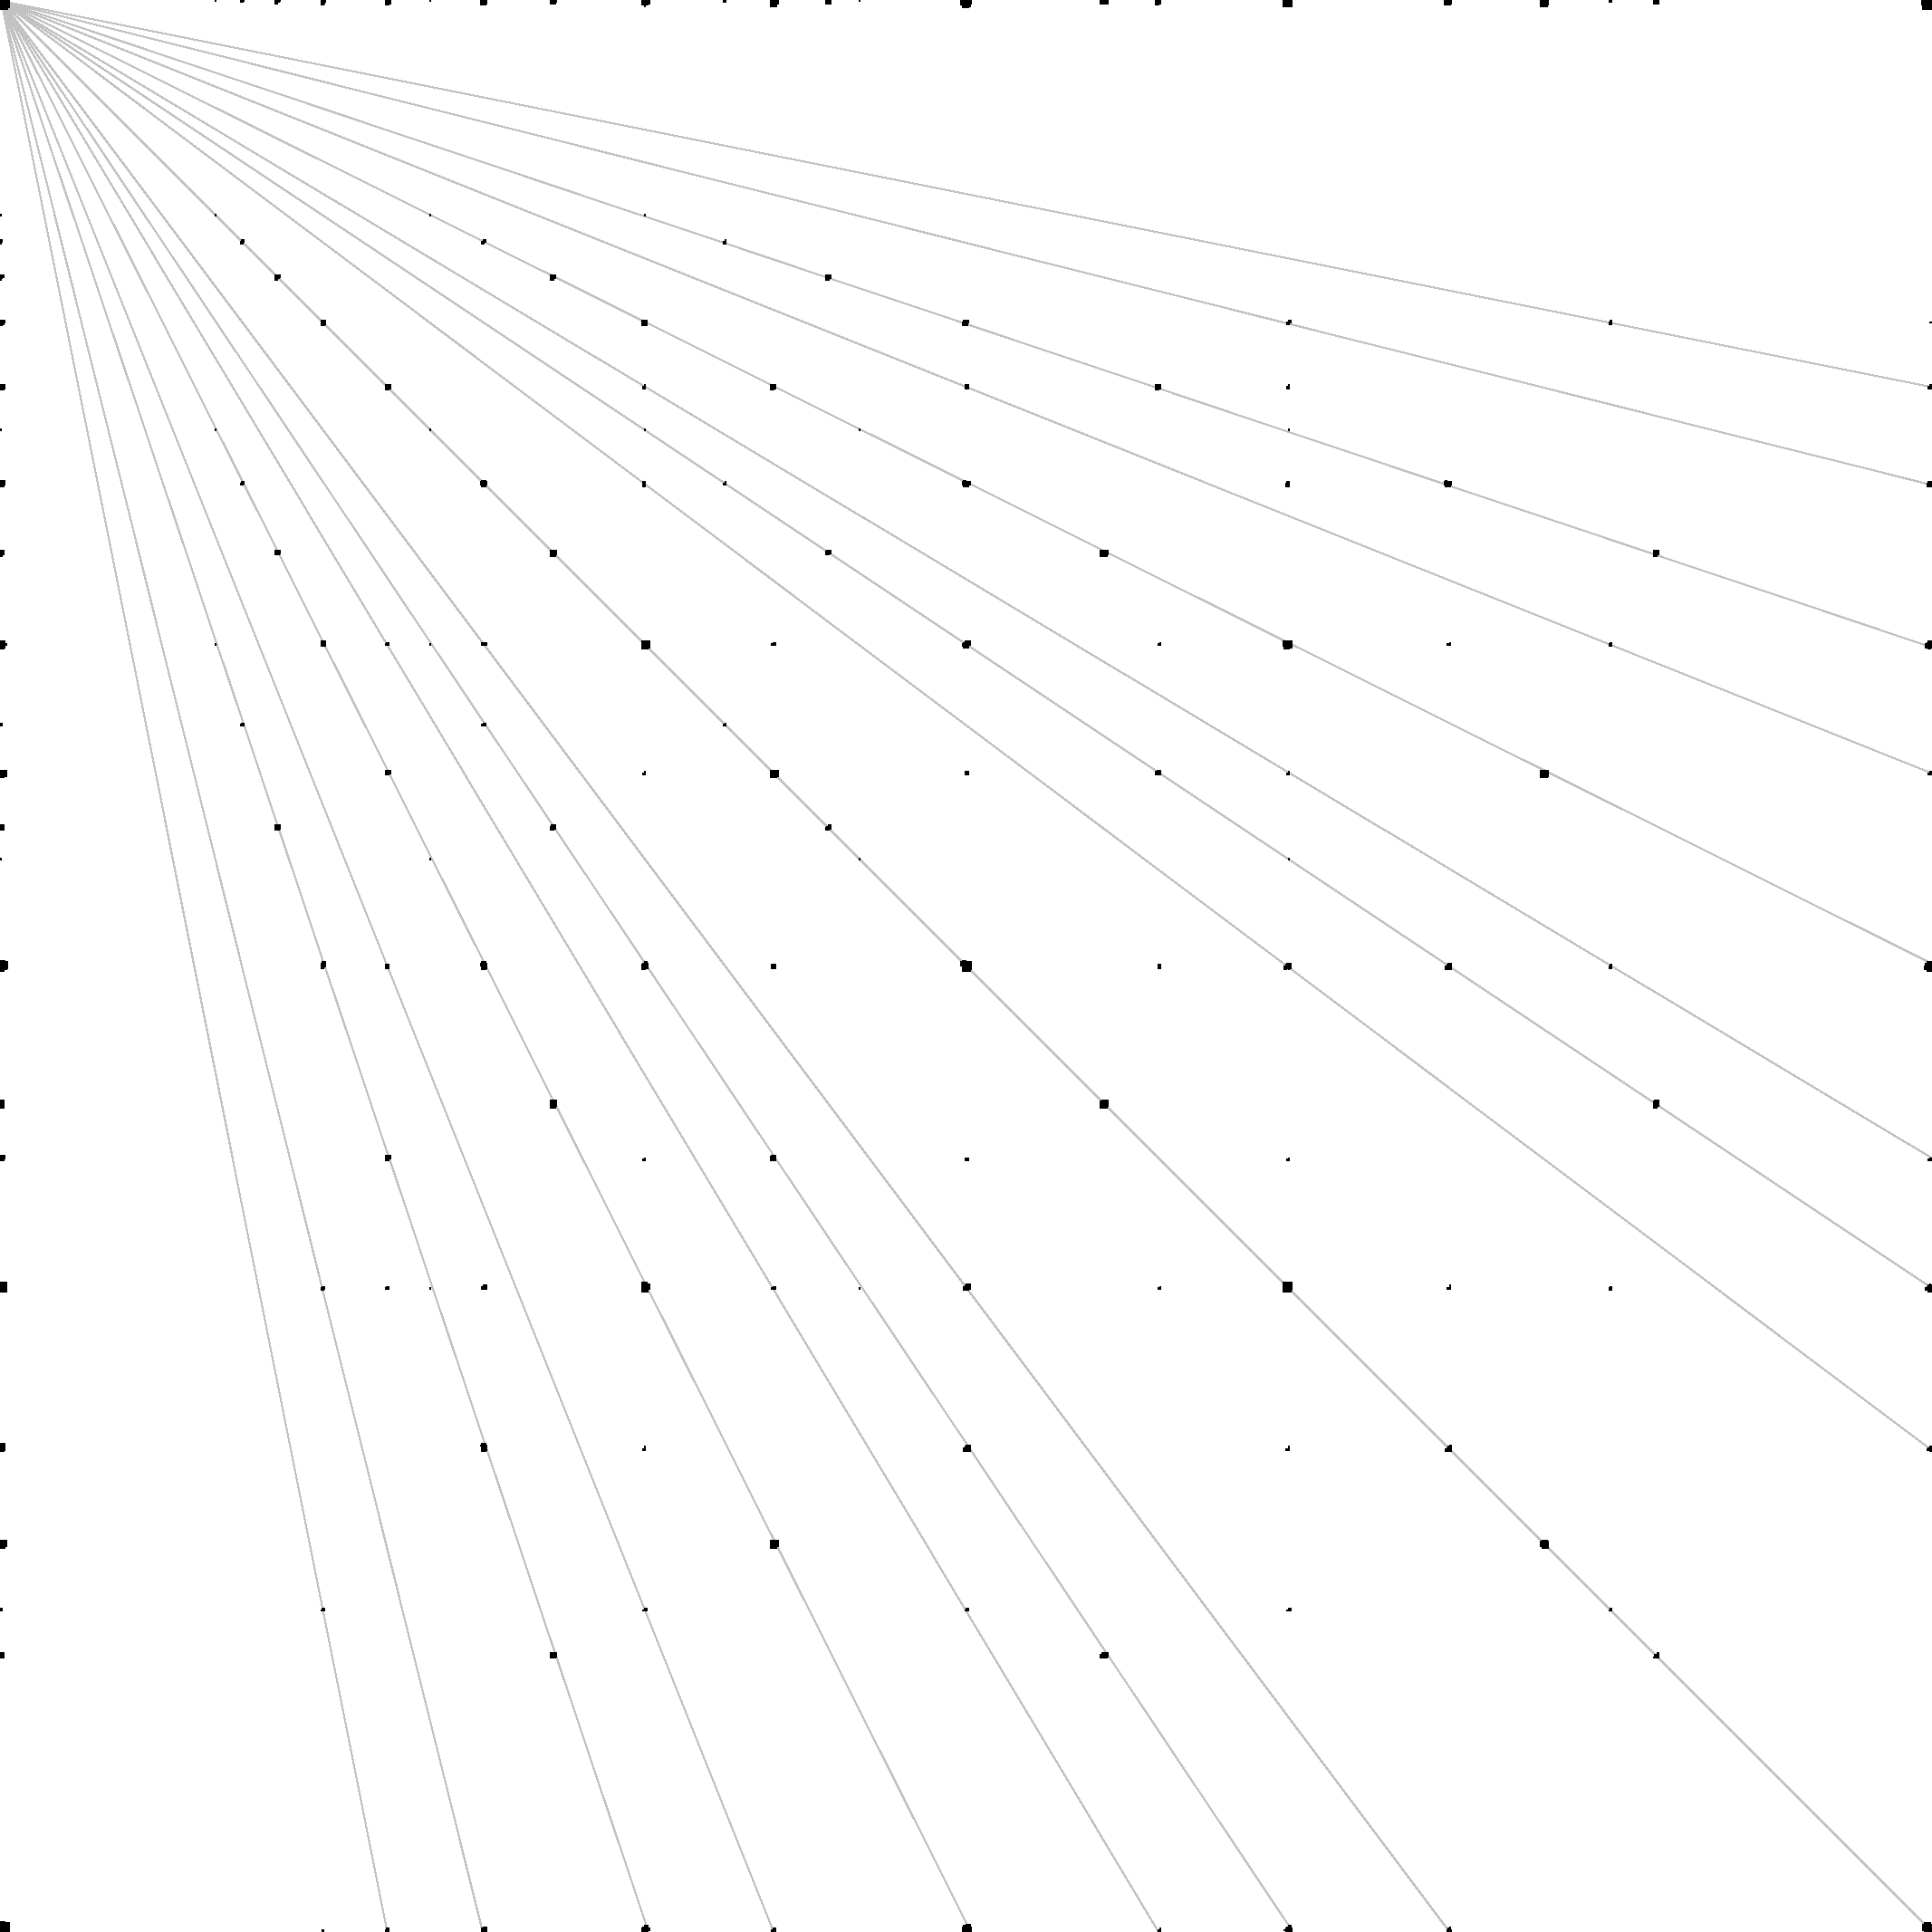
\includegraphics[width=0.90 \linewidth]{powerday3.pdf}
\end{center}\vspace{-0.1in}
\caption{All possible outcomes for the first two players in 3-player
  power days. These are the same games as the 3-player power hours,
  but at this scale makes it clear the groupings and their sparsity
  in the limit. Lines plotted from (0,0) to (60,*) and (*,60) show
  significant structure, but don't explain some of the interior points.
  (TODO: what are these games? what did the other player drink?)
}
\label{fig:powerday3}
\end{figure}

\section{Some stuffff}

Hi

\end{document}
